\chapter{PCB相关资料}
\label{cha:Appendix-PCB}

\section{Mega2560引脚映射}
\label{sec:Pin2560}
% Please add the following required packages to your document preamble:
% \usepackage{longtable}
% Note: It may be necessary to compile the document several times to get a multi-page table to line up properly
\begin{longtable}[c]{|l|l|l|}
    \hline
    Pin Number & Pin Name                 & Mapped Pin Name       \\ \hline
    \endfirsthead
    %
    \endhead
    %
    1          & PG5 ( OC0B )             & Digital pin 4 (PWM)   \\ \hline
    2          & PE0 ( RXD0/PCINT8 )      & Digital pin 0 (RX0)   \\ \hline
    3          & PE1 ( TXD0 )             & Digital pin 1 (TX0)   \\ \hline
    4          & PE2 ( XCK0/AIN0 )        &                       \\ \hline
    5          & PE3 ( OC3A/AIN1 )        & Digital pin 5 (PWM)   \\ \hline
    6          & PE4 ( OC3B/INT4 )        & Digital pin 2 (PWM)   \\ \hline
    7          & PE5 ( OC3C/INT5 )        & Digital pin 3 (PWM)   \\ \hline
    8          & PE6 ( T3/INT6 )          &                       \\ \hline
    9          & PE7 ( CLKO/ICP3/INT7 )   &                       \\ \hline
    10         & VCC                      & VCC                   \\ \hline
    11         & GND                      & GND                   \\ \hline
    12         & PH0 ( RXD2 )             & Digital pin 17 (RX2)  \\ \hline
    13         & PH1 ( TXD2 )             & Digital pin 16 (TX2)  \\ \hline
    14         & PH2 ( XCK2 )             &                       \\ \hline
    15         & PH3 ( OC4A )             & Digital pin 6 (PWM)   \\ \hline
    16         & PH4 ( OC4B )             & Digital pin 7 (PWM)   \\ \hline
    17         & PH5 ( OC4C )             & Digital pin 8 (PWM)   \\ \hline
    18         & PH6 ( OC2B )             & Digital pin 9 (PWM)   \\ \hline
    19         & PB0 ( SS/PCINT0 )        & Digital pin 53 (SS)   \\ \hline
    20         & PB1 ( SCK/PCINT1 )       & Digital pin 52 (SCK)  \\ \hline
    21         & PB2 ( MOSI/PCINT2 )      & Digital pin 51 (MOSI) \\ \hline
    22         & PB3 ( MISO/PCINT3 )      & Digital pin 50 (MISO) \\ \hline
    23         & PB4 ( OC2A/PCINT4 )      & Digital pin 10 (PWM)  \\ \hline
    24         & PB5 ( OC1A/PCINT5 )      & Digital pin 11 (PWM)  \\ \hline
    25         & PB6 ( OC1B/PCINT6 )      & Digital pin 12 (PWM)  \\ \hline
    26         & PB7 ( OC0A/OC1C/PCINT7 ) & Digital pin 13 (PWM)  \\ \hline
    27         & PH7 ( T4 )               &                       \\ \hline
    28         & PG3 ( TOSC2 )            &                       \\ \hline
    29         & PG4 ( TOSC1 )            &                       \\ \hline
    30         & RESET                    & RESET                 \\ \hline
    31         & VCC                      & VCC                   \\ \hline
    32         & GND                      & GND                   \\ \hline
    33         & XTAL2                    & XTAL2                 \\ \hline
    34         & XTAL1                    & XTAL1                 \\ \hline
    35         & PL0 ( ICP4 )             & Digital pin 49        \\ \hline
    36         & PL1 ( ICP5 )             & Digital pin 48        \\ \hline
    37         & PL2 ( T5 )               & Digital pin 47        \\ \hline
    38         & PL3 ( OC5A )             & Digital pin 46 (PWM)  \\ \hline
    39         & PL4 ( OC5B )             & Digital pin 45 (PWM)  \\ \hline
    40         & PL5 ( OC5C )             & Digital pin 44 (PWM)  \\ \hline
    41         & PL6                      & Digital pin 43        \\ \hline
    42         & PL7                      & Digital pin 42        \\ \hline
    43         & PD0 ( SCL/INT0 )         & Digital pin 21 (SCL)  \\ \hline
    44         & PD1 ( SDA/INT1 )         & Digital pin 20 (SDA)  \\ \hline
    45         & PD2 ( RXDI/INT2 )        & Digital pin 19 (RX1)  \\ \hline
    46         & PD3 ( TXD1/INT3 )        & Digital pin 18 (TX1)  \\ \hline
    47         & PD4 ( ICP1 )             &                       \\ \hline
    48         & PD5 ( XCK1 )             &                       \\ \hline
    49         & PD6 ( T1 )               &                       \\ \hline
    50         & PD7 ( T0 )               & Digital pin 38        \\ \hline
    51         & PG0 ( WR )               & Digital pin 41        \\ \hline
    52         & PG1 ( RD )               & Digital pin 40        \\ \hline
    53         & PC0 ( A8 )               & Digital pin 37        \\ \hline
    54         & PC1 ( A9 )               & Digital pin 36        \\ \hline
    55         & PC2 ( A10 )              & Digital pin 35        \\ \hline
    56         & PC3 ( A11 )              & Digital pin 34        \\ \hline
    57         & PC4 ( A12 )              & Digital pin 33        \\ \hline
    58         & PC5 ( A13 )              & Digital pin 32        \\ \hline
    59         & PC6 ( A14 )              & Digital pin 31        \\ \hline
    60         & PC7 ( A15 )              & Digital pin 30        \\ \hline
    61         & VCC                      & VCC                   \\ \hline
    62         & GND                      & GND                   \\ \hline
    63         & PJ0 ( RXD3/PCINT9 )      & Digital pin 15 (RX3)  \\ \hline
    64         & PJ1 ( TXD3/PCINT10 )     & Digital pin 14 (TX3)  \\ \hline
    65         & PJ2 ( XCK3/PCINT11 )     &                       \\ \hline
    66         & PJ3 ( PCINT12 )          &                       \\ \hline
    67         & PJ4 ( PCINT13 )          &                       \\ \hline
    68         & PJ5 ( PCINT14 )          &                       \\ \hline
    69         & PJ6 ( PCINT 15 )         &                       \\ \hline
    70         & PG2 ( ALE )              & Digital pin 39        \\ \hline
    71         & PA7 ( AD7 )              & Digital pin 29        \\ \hline
    72         & PA6 ( AD6 )              & Digital pin 28        \\ \hline
    73         & PA5 ( AD5 )              & Digital pin 27        \\ \hline
    74         & PA4 ( AD4 )              & Digital pin 26        \\ \hline
    75         & PA3 ( AD3 )              & Digital pin 25        \\ \hline
    76         & PA2 ( AD2 )              & Digital pin 24        \\ \hline
    77         & PA1 ( AD1 )              & Digital pin 23        \\ \hline
    78         & PA0 ( AD0 )              & Digital pin 22        \\ \hline
    79         & PJ7                      &                       \\ \hline
    80         & VCC                      & VCC                   \\ \hline
    81         & GND                      & GND                   \\ \hline
    82         & PK7 ( ADC15/PCINT23 )    & Analog pin 15         \\ \hline
    83         & PK6 ( ADC14/PCINT22 )    & Analog pin 14         \\ \hline
    84         & PK5 ( ADC13/PCINT21 )    & Analog pin 13         \\ \hline
    85         & PK4 ( ADC12/PCINT20 )    & Analog pin 12         \\ \hline
    86         & PK3 ( ADC11/PCINT19 )    & Analog pin 11         \\ \hline
    87         & PK2 ( ADC10/PCINT18 )    & Analog pin 10         \\ \hline
    88         & PK1 ( ADC9/PCINT17 )     & Analog pin 9          \\ \hline
    89         & PK0 ( ADC8/PCINT16 )     & Analog pin 8          \\ \hline
    90         & PF7 ( ADC7/TDI )         & Analog pin 7          \\ \hline
    91         & PF6 ( ADC6/TDO )         & Analog pin 6          \\ \hline
    92         & PF5 ( ADC5/TMS )         & Analog pin 5          \\ \hline
    93         & PF4 ( ADC4/TCK )         & Analog pin 4          \\ \hline
    94         & PF3 ( ADC3 )             & Analog pin 3          \\ \hline
    95         & PF2 ( ADC2 )             & Analog pin 2          \\ \hline
    96         & PF1 ( ADC1 )             & Analog pin 1          \\ \hline
    97         & PF0 ( ADC0 )             & Analog pin 0          \\ \hline
    98         & AREF                     & Analog Reference      \\ \hline
    99         & GND                      & GND                   \\ \hline
    100        & AVCC                     & VCC                   \\ \hline
    \caption{Arduino Mega 2560 PIN mapping table}
    \label{tab:PinMap}\\
\end{longtable}

\section{ESP32-WROOM-32管脚定义}

\includepdf[pages={8-9}]{esp32-wroom-32_datasheet_cn.pdf}

\section{PCB原理图}
% ! LaTeX Error: Cannot determine size of graphic in figures/Misaka-v1.0.pdf (no BoundingBox).
% 解决:去掉Misaka-v1.0.pdf的.0。在文件名中不能出现点。

% xdvipdfmx:fatal: pdf_ref_obj(): passed invalid object.   This happened to me when embedding an EPS file into a xelatex document.
% 未解决,可能是Misaka-v1.pdf有点问题
% 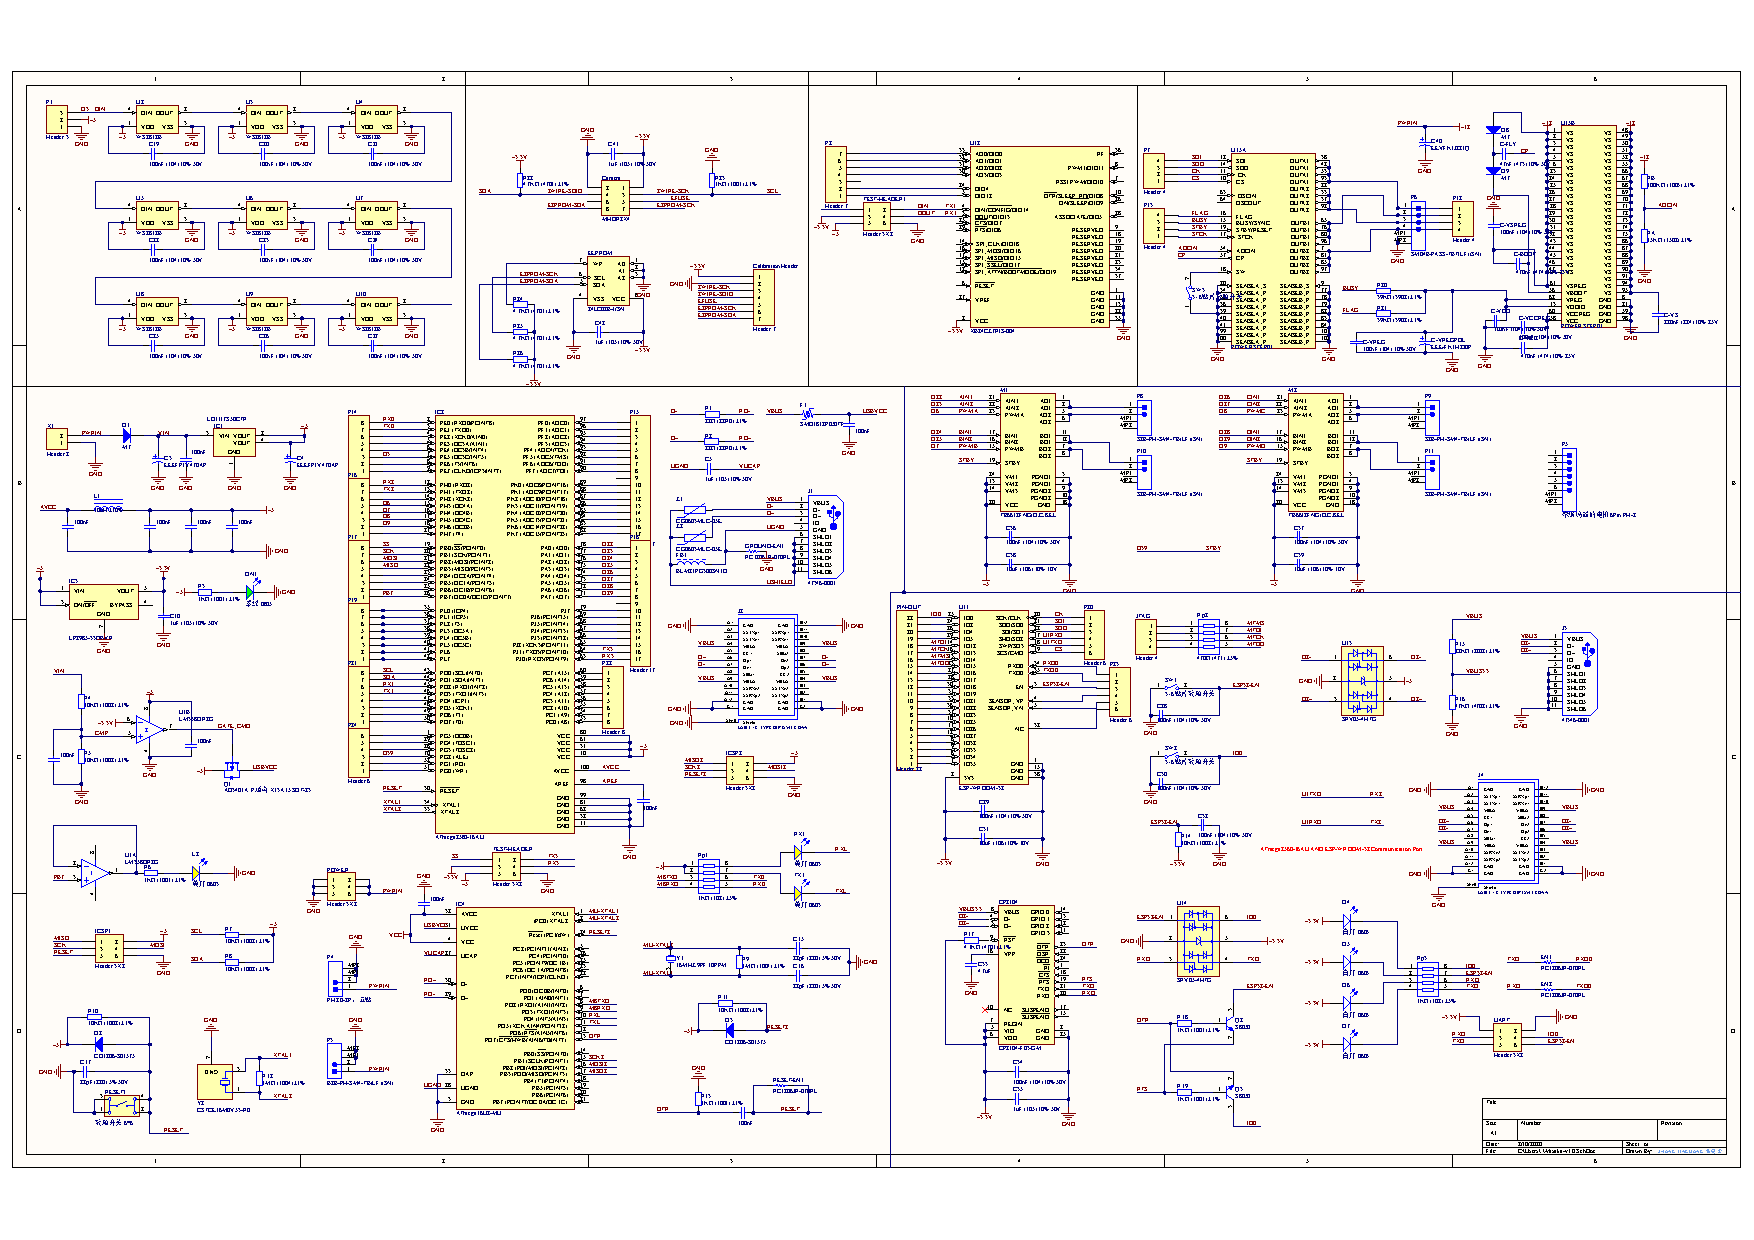
\includepdf[pages={1-2}]{Misaka-v1.pdf} 

% 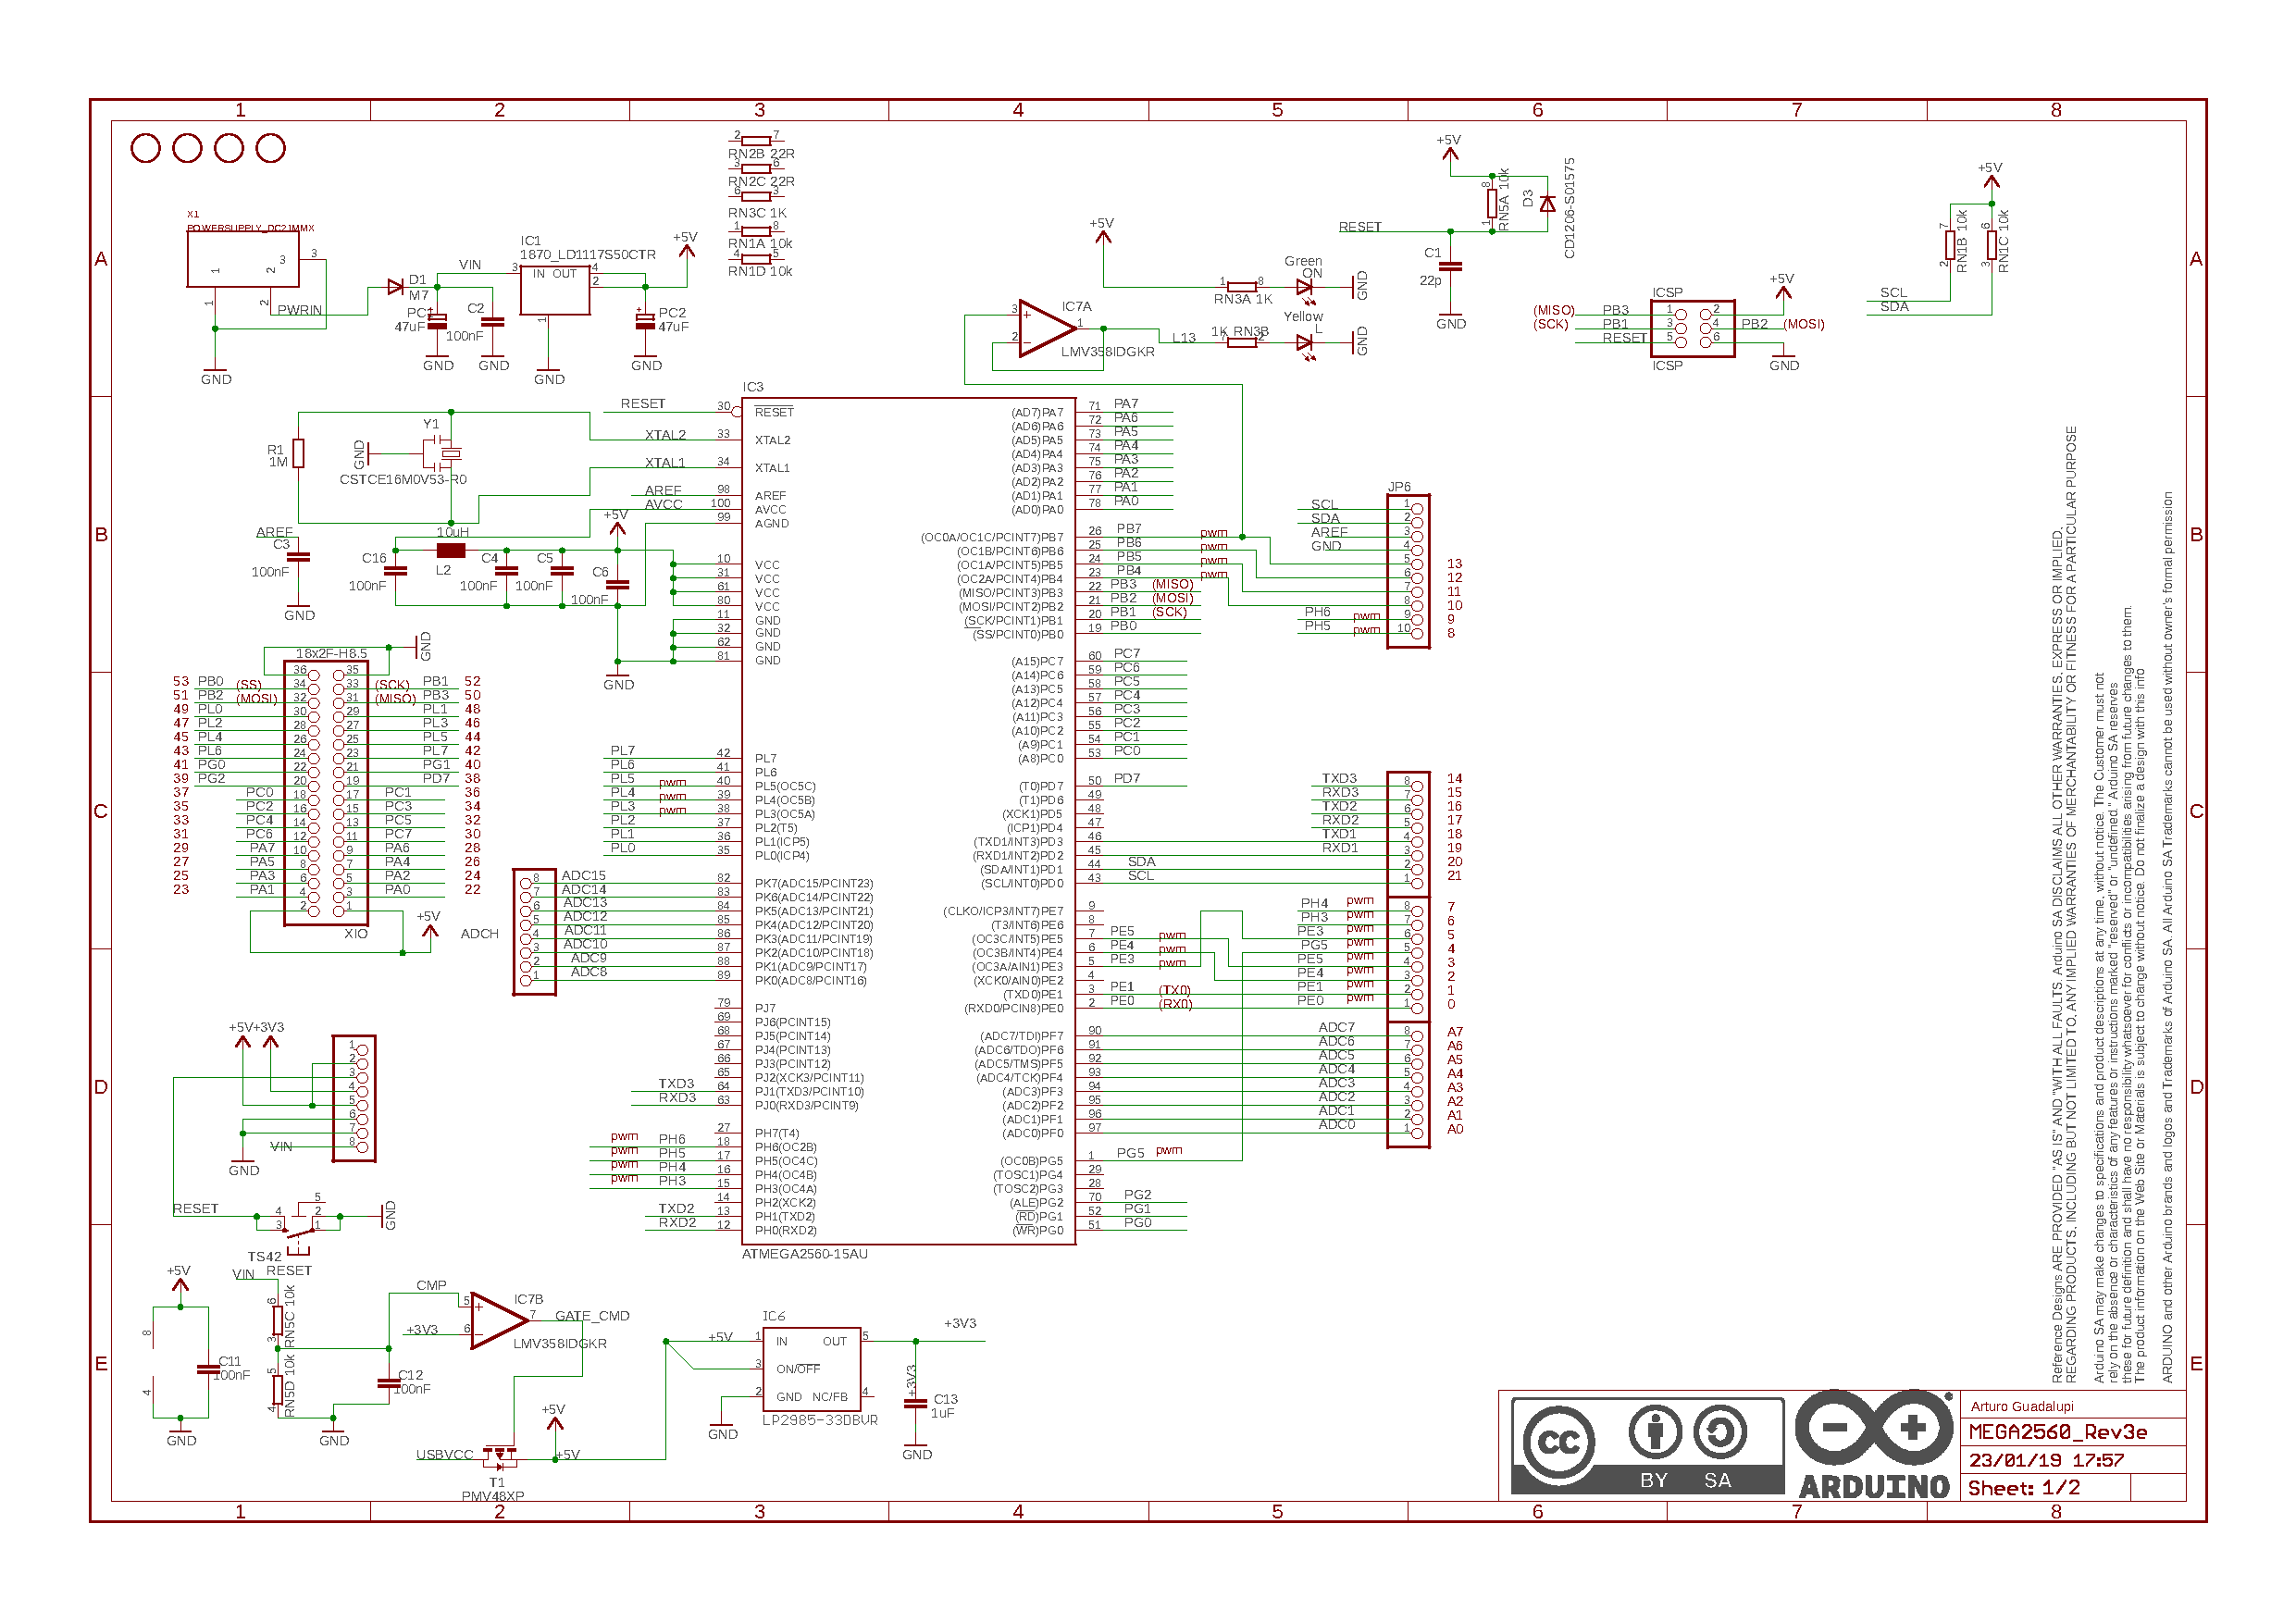
\includepdf[pages={1-2}]{MEGA2560_Rev3e_sch.pdf}
% 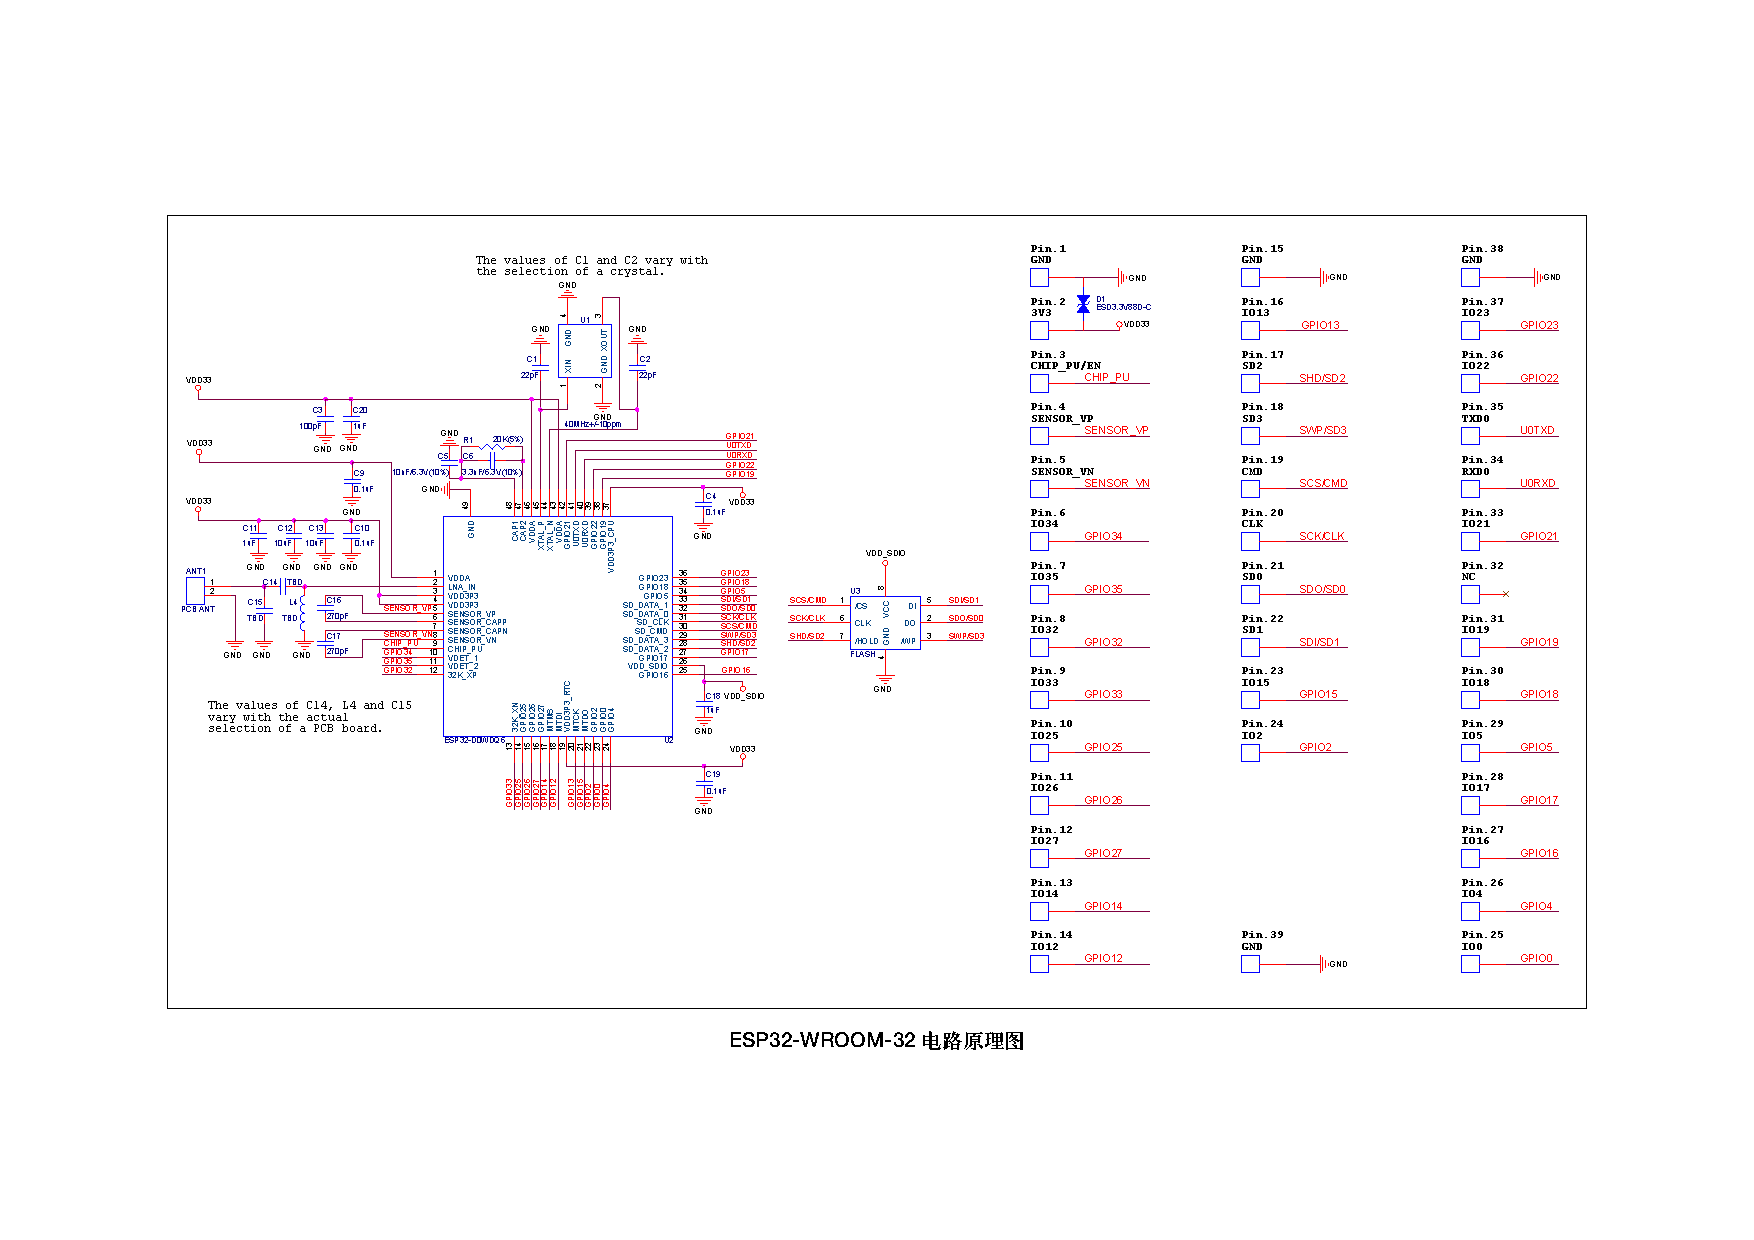
\includepdf[]{esp32-wroom-32_datasheet_cn_Inside.pdf}
% 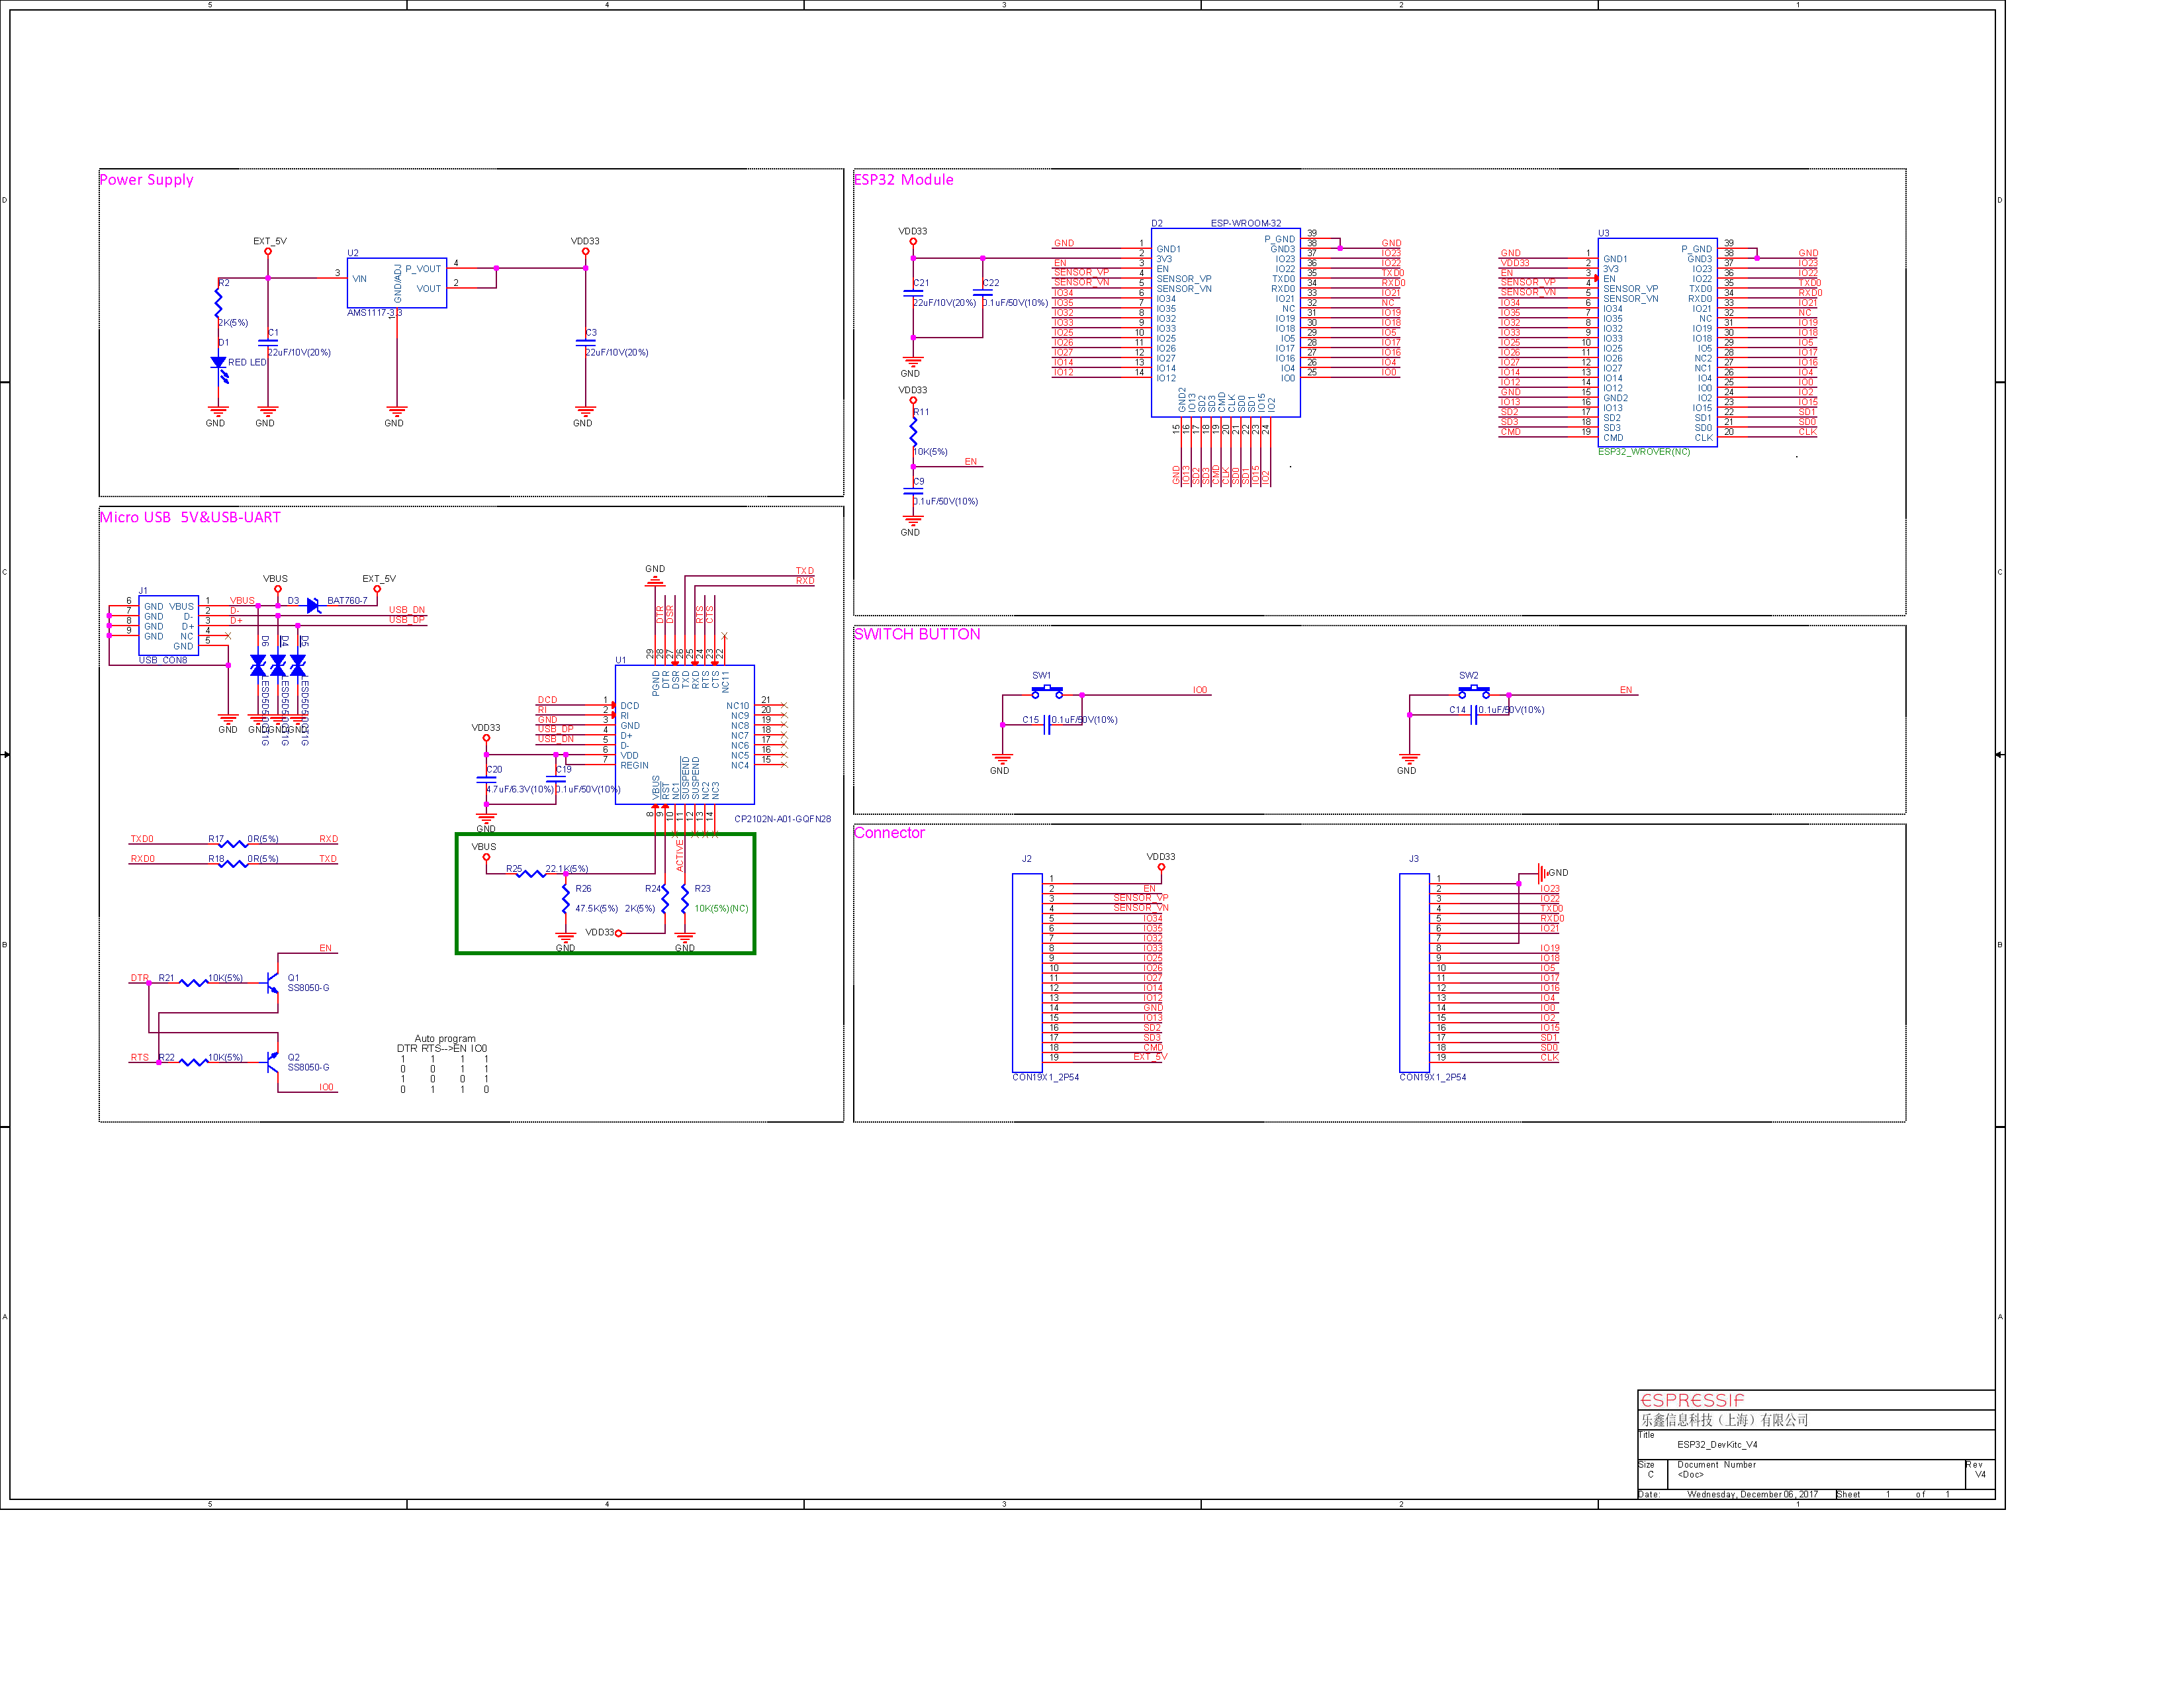
\includepdf[]{esp32_devkitc_v4-sch.pdf}
% 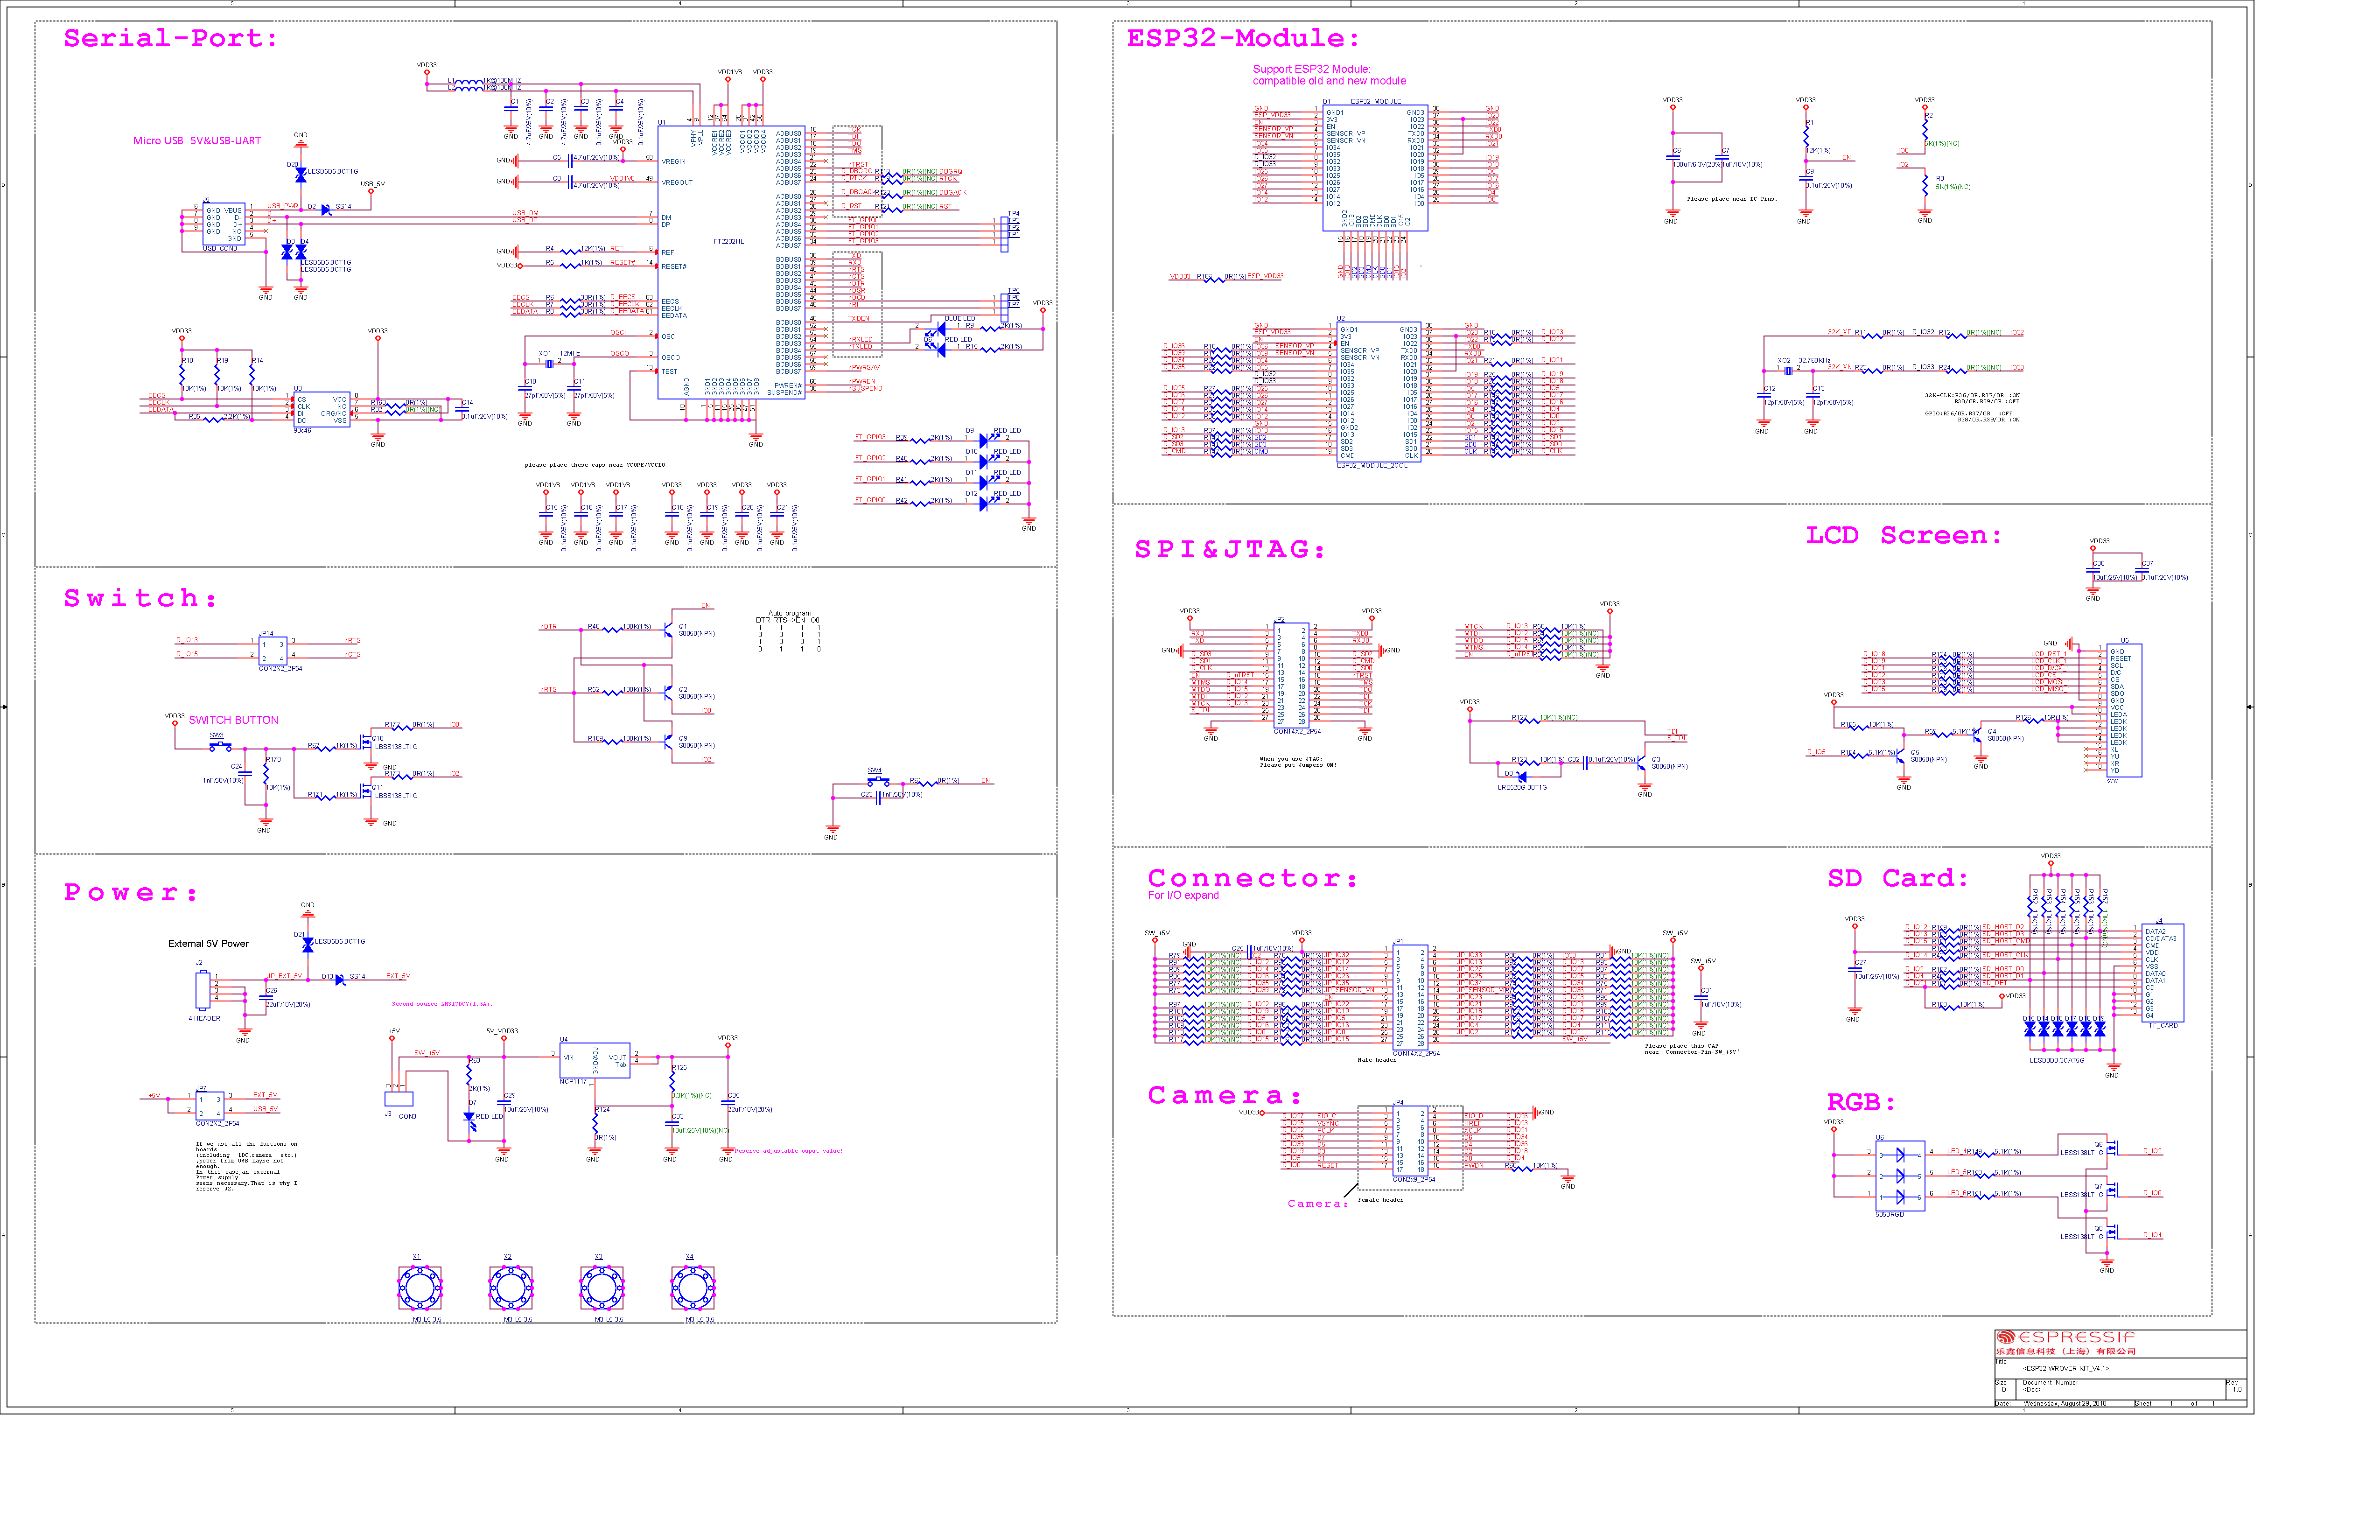
\includepdf[]{ESP-WROVER-KIT_V4_1.pdf}